% 2004 福建文科第16题：正六边形铁皮切角折成正六棱柱
% 外层实线正六边形边长按图取 1，内层虚线正六边形边长 x=2/3；六个角为全等灰色四边形。
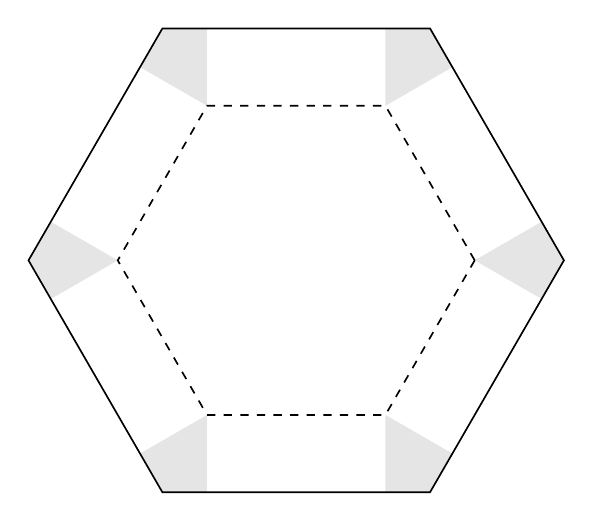
\begin{tikzpicture}[x=1cm,y=1cm,line width=.6pt,font=\normalsize]
\coordinate (O) at (0,0);
\coordinate (V0) at (3.400000,0.000000);
\coordinate (V1) at (1.700000,2.944486);
\coordinate (V2) at (-1.700000,2.944486);
\coordinate (V3) at (-3.400000,0.000000);
\coordinate (V4) at (-1.700000,-2.944486);
\coordinate (V5) at (1.700000,-2.944486);
\coordinate (W0) at (2.266667,0.000000);
\coordinate (W1) at (1.133333,1.962991);
\coordinate (W2) at (-1.133333,1.962991);
\coordinate (W3) at (-2.266667,0.000000);
\coordinate (W4) at (-1.133333,-1.962991);
\coordinate (W5) at (1.133333,-1.962991);
\coordinate (A0) at (3.116667,0.490748);
\coordinate (A1) at (1.133333,2.944486);
\coordinate (A2) at (-1.983333,2.453739);
\coordinate (A3) at (-3.116667,-0.490748);
\coordinate (A4) at (-1.133333,-2.944486);
\coordinate (A5) at (1.983333,-2.453739);
\coordinate (B0) at (3.116667,-0.490748);
\coordinate (B1) at (1.983333,2.453739);
\coordinate (B2) at (-1.133333,2.944486);
\coordinate (B3) at (-3.116667,0.490748);
\coordinate (B4) at (-1.983333,-2.453739);
\coordinate (B5) at (1.133333,-2.944486);
% 六个全等切角四边形，仅填充，无内部描边
\fill[black!10] (V0)--(A0)--(W0)--(B0)--cycle;
\fill[black!10] (V1)--(A1)--(W1)--(B1)--cycle;
\fill[black!10] (V2)--(A2)--(W2)--(B2)--cycle;
\fill[black!10] (V3)--(A3)--(W3)--(B3)--cycle;
\fill[black!10] (V4)--(A4)--(W4)--(B4)--cycle;
\fill[black!10] (V5)--(A5)--(W5)--(B5)--cycle;
% 外轮廓
\draw (V0)--(V1)--(V2)--(V3)--(V4)--(V5)--cycle;
% 内层折线（底面正六边形）
\draw[dashed] (W0)--(W1)--(W2)--(W3)--(W4)--(W5)--cycle;
\end{tikzpicture}
